\documentclass[11pt, a4paper]{article} 

\usepackage[14pt]{extsizes}
\usepackage{amsmath}
\usepackage[left=2cm,right=2cm,top=1cm,bottom=1cm,bindingoffset=0cm]{geometry}
\usepackage{fontspec} % loaded by polyglossia, but included here for transparency 
\usepackage{polyglossia}
\usepackage{xspace}
\usepackage{todonotes}
\usepackage{graphicx}
\graphicspath{ {./images/} }
\usepackage{hyperref}
\hypersetup{
    colorlinks=true,
    linkcolor=blue,
    filecolor=magenta,      
    urlcolor=blue,
}
\usepackage{listings}
\usepackage{xcolor}

 
\definecolor{codegreen}{rgb}{0,0.6,0}
\definecolor{codegray}{rgb}{0.5,0.5,0.5}
\definecolor{codepurple}{rgb}{0.58,0,0.82}
\definecolor{backcolour}{rgb}{0.95,0.95,0.92}
 
\lstdefinestyle{mystyle}{
    backgroundcolor=\color{backcolour},   
    commentstyle=\color{codegreen},
    keywordstyle=\color{magenta},
    numberstyle=\tiny\color{codegray},
    stringstyle=\color{codepurple},
    basicstyle=\ttfamily\footnotesize,
    breakatwhitespace=false,         
    breaklines=true,                 
    captionpos=b,                    
    keepspaces=true,                 
    numbers=left,                    
    numbersep=5pt,                  
    showspaces=false,                
    showstringspaces=false,
    showtabs=false,                  
    tabsize=2
}
 
\lstset{style=mystyle}

\newfontfamily{\cyrillicfont}{Times New Roman} 
\newfontfamily{\cyrillicfonttt}{Courier New}
\newfontfamily{\cyrillicfontsf}{Arial}
\setmainlanguage{russian} 
\setotherlanguage{turkish}

\title{Шаблон русского документа \LaTeX}
\author{Иван Сошников}

\begin{document}

\maketitle

\tableofcontents

\listoftodos

\pagebreak

\section{Раздел. Глава.}

\todo{Тудушка}

\subsection{Подраздел}

\begin{figure}[h]
\centering
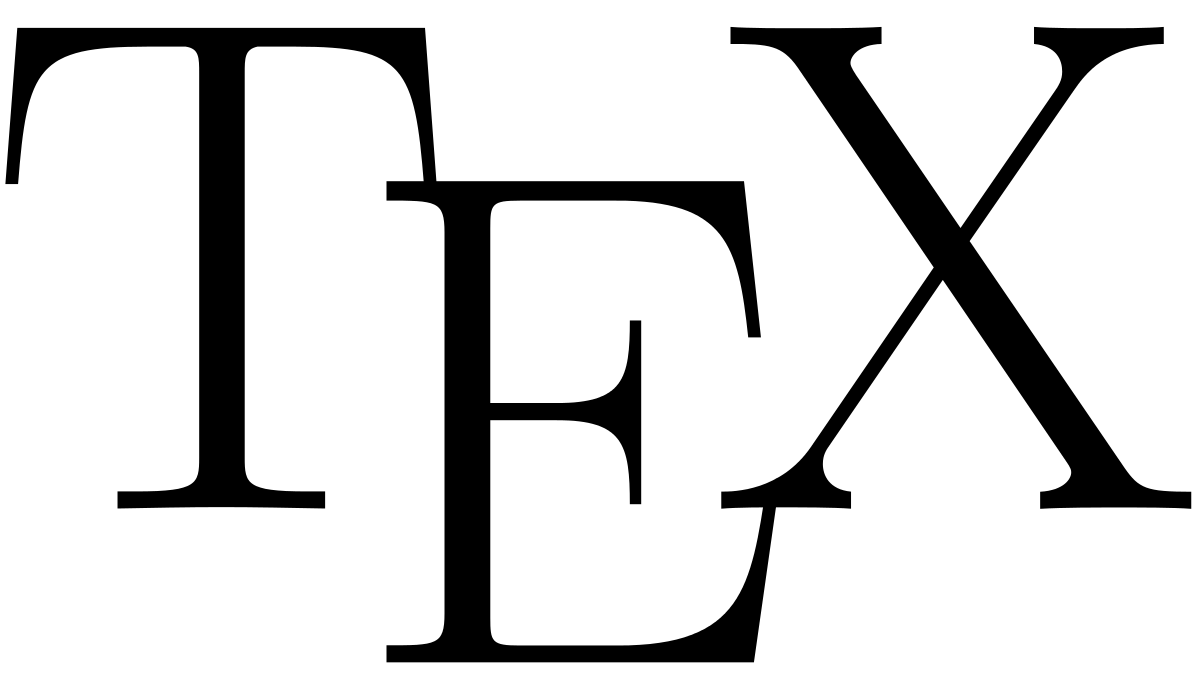
\includegraphics[scale=.2]{tex_logo}
\caption{Пример картинки}
\end{figure}

\begin{itemize}
	\setlength\itemsep{-.6em}
	\item Элемент списка
	\item Элемент списка
\end{itemize}

\begin{table}[h]
	\centering
	\begin{tabular}{|l|l|}
	\hline
	1 -е лицо единственное число & -m/-ım/-im/-um/-üm \\ \hline
	1-е лицо множественное число & -ız/-iz/-uz/-üz/-yız/- yiz/-yuz/-yüz \\ \hline
	2-е лицо единственное число & -sın/-sin/-sun/sün \\ \hline
	2-е лицо множественное число & -sınız/-siniz/-sunuz/ sünüz \\ \hline
	3-е лицо единственное число & нулевой суффикс \\ \hline
	3-е лицо множественное число & -lar/-ler \\ \hline
	\end{tabular}
	\caption{Пример таблички}
\end{table}

\end{document}